\documentclass[12pt,a4paper,oneside]{book}

\usepackage{graphicx}
\usepackage{amsmath}
\usepackage{amsfonts}
\usepackage{mathtools}
\usepackage{amsthm}
\usepackage{amssymb}
\usepackage{newlfont}
\usepackage{listings}
\usepackage{xcolor}
\usepackage{comment}
\usepackage{algorithm}
\usepackage{algpseudocode}
\usepackage[italian]{babel}

% TODO QUI È DOVE INIZIA LA DEFINIZIONE DELLE SCRITTURE DI CODICE

\definecolor{codegreen}{rgb}{0,0.6,0}
\definecolor{codegray}{rgb}{0.5,0.5,0.5}
\definecolor{codepurple}{rgb}{0.58,0,0.82}
\definecolor{backcolour}{rgb}{0.95,0.95,0.92}

\lstdefinestyle{mystyle}{
	backgroundcolor=\color{backcolour},   
	commentstyle=\color{codegreen},
	keywordstyle=\color{magenta},
	numberstyle=\tiny\color{codegray},
	stringstyle=\color{codepurple},
	basicstyle=\ttfamily\footnotesize,
	breakatwhitespace=false,         
	breaklines=true,                 
	captionpos=b,                    
	keepspaces=true,                 
	numbers=left,                    
	numbersep=5pt,                  
	showspaces=false,                
	showstringspaces=false,
	showtabs=false,                  
	tabsize=2
}

\lstset{style=mystyle}
\makeatother

\newtheorem{theorem}{Teorema}
\newtheorem{definition}{Definizione}
\newtheorem{eg}{Esempio}
\newcommand*{\blankpage}{
{\newpage \vspace*{5cm}\thispagestyle{empty}\centering \bfseries  \textit{Inserire citazione inerente alla materia}\par}
\vspace{\fill}}

\textwidth=450pt\oddsidemargin=0pt

\begin{document}
	
	\begin{titlepage}
		\begin{center}
			{{\LARGE{\textsc{Università degli Studi di Verona}}}} \rule[0.1cm]{15.8cm}{0.1mm}
			\rule[0.5cm]{15.8cm}{0.6mm}
			{\small{\bf CORSO DI LAUREA IN INFORMATICA }}
		\end{center}
		\vspace{12.5mm}
		
		\begin{center}
			{\Huge{\bf Intelligenza Artificiale}}
		\end{center}
		\vspace{130mm}
		
		\begin{minipage}[l]{1.8mm}
			\rule[0.1cm]{0.1mm}{2cm}
			\rule[0.1cm]{0.6mm}{2cm}
		\end{minipage}
		\hspace{2mm}
		\begin{minipage}{10cm}	
			{\large{Federico Brutti\\
			\texttt{federico.brutti@studenti.univr.it}}}
		\end{minipage}
	\end{titlepage}
	
	\blankpage
	\tableofcontents
	
	\chapter{Agenti intelligenti}
	\section{Agenti e razionalità}
Il campo dell'\textbf{intelligenza artificiale} ha lo scopo di comprendere e creare entità intelligenti, macchine capaci di calcolare come agire in modo
efficace e sicuro in base alla situazione presa in esame. Si tratta di una disciplina molto ampia e suddivisa in un gran numero di sottoinsiemi; alcuni
di questi, come l'apprendimento e la percezione, sono ambiti generali, mentre in altre diramazioni si applica l'AI anche per problemi specifici, come la
dimostrazione di teoremi matematici. Esistono più scuole di pensiero riguardanti la definizione formale di "intelligenza"; una prima idea, che ha
origine dalla psicologia, vede più intelligenti quelle entità capaci di rispecchiare al meglio la mente umana, ma tendenzialmente si preferisce usare
la nozione di \textbf{razionalità}, ovvero, dato un problema particolare, di compiere un'azione corretta per avvicinarsi alla sua risoluzione.\par
Le entità usate in questa disciplina si chiamano \textbf{Agenti}, i quali rappresentano un sistema capace di percepire il suo ambiente attraverso dei
\textbf{sensori} e agisce su di esso mediante \textbf{attuatori}; non dissimilmente da come una persona percepisce e interagisce con ciò che lo circonda.
In particolare, i dati percepiti dagli agenti formano una \textbf{sequenza percettiva}, ovvero lo storico di quanto da essi osservato all'interno del
loro ambiente. Il comportamento di un agente è poi descritto da una \textbf{funzione agente}, la quale mostra la corrispondenza tra una qualsiasi
sequenza percettiva e una specifica azione, ed è implementata dal \textbf{programma agente}, un algoritmo in esecuzione all'interno del sistema
fisico.\par
Potendo inserire diversi algoritmi usati come programma agente, è necessario capire in che modo determinare quando un agente è adatto al compito che gli
è richiesto di eseguire. Richiamando il precedente concetto, definiamo \textbf{agenti razionali} quei sistemi che eseguono un'azione "corretta", atta
alla risoluzione del problema, la quale è valutata in base a una \textbf{misura di prestazione}, il criterio per definire quanto efficaci siano state.
In questi termini, è auspicabile massimizzare il valore atteso da questa misura per ogni sequenza percettiva ottenibile, mostrando come la qualità di
un agente sia un problema di ottimizzazione.
\begin{figure}[h]
    \centering
    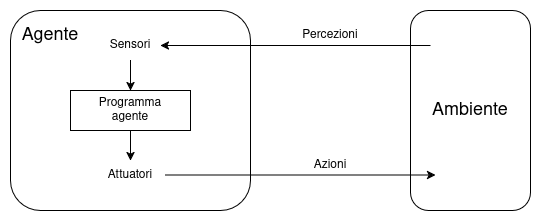
\includegraphics[width=0.8\linewidth]{Images/Agent.png}
    \caption{Struttura di un agente}    
\end{figure}

\noindent Supponiamo per esempio un ambiente composto da due stanze sporche e l'obiettivo è pulirle tutte. Si potrebbe usare il seguente programma
agente per rimuovere lo sporco: \begin{algorithm}[h]
    \caption{Reflex-Vacuum-Agent(location, status) \textbf{returns} action}
    \begin{algorithmic}[i]
         \If{status = dirty} \textbf{return} Suck
         \ElsIf{location = A} \textbf{return} Right
         \ElsIf{location = B} \textbf{return} Left
         \EndIf
    \end{algorithmic}
\end{algorithm}

\noindent Se l'unica misura di prestazione è la pulizia dell'ambiente, possiamo dire che questo agente è razionale e buono, ma se si aggiungessero
ulteriori condizioni sarà necessario rivedere l'algoritmo utilizzato. È comune, in problemi come questo, usare come misura il valore di \textbf{average
idleness}, la somma degli intervalli di tempo per i quali l'agente non visita altri stati, per poterla minimizzare e risolvere il problema il prima
possibile. In questi termini è desiderabile considerare tutti gli stati allo stesso modo, con lo scopo di ottenere valori medi i più omogenei possibile.
Ciò si traduce nel cercare di minimizzare il valore di varianza, siccome più basso sarà, tanto più omogenei saranno i valori di idleness.

%

\section{Struttura degli agenti}
Ora che abbiamo compreso le componenti che formano gli agenti razionali, è necessario fornire una visione più formale di cosa definire per poterli
progettare al meglio. Gli elementi sono dati dall'acronimo \textbf{PEAS}, ovvero: \begin{itemize}
    \item \textbf{Performance measure}: Risultato desiderato dall'agente.
    \item \textbf{Environment}: Ambiente di lavoro al quale è applicato l'agente.
    \item \textbf{Actuators}: Elementi che definiscono come l'agente può compiere azioni.
    \item \textbf{Sensors}: Elementi che definiscono come l'agente è in grado di percepire l'ambiente.
\end{itemize}

\noindent Esistono inoltre diversi tipi di ambienti con una struttura condivisa per poter definire il tipo di problema preso in esame. È di fondamentale
importanza conoscerli a fondo poiché il design degli algoritmi si baserà in gran parte su di essi: \begin{itemize}
    \item \textbf{Osservabile}: Lo stato del mondo è completamente visibile dall'agente.
    \item \textbf{Deterministico}: Le azioni hanno conseguenze perfettamente predicibili dall'agente.
    \item \textbf{Episodico}: Le azioni che l'agente compie impattano esclusivamente la sola istanza di lavoro corrente. Ciò non fa cambiare strategia.
    \item \textbf{Statico}: Si lavora sempre nello stesso ambiente non modificabile; solo le azioni dell'agente potranno cambiare.
    \item \textbf{Discreto}: Il problema è esprimibile con sole variabili discrete.
    \item \textbf{A singolo agente}: Il problema presenta l'utilizzo di un singolo agente.
\end{itemize}

\noindent In base al tipo di problema proposto, si tenderà a cadere in uno dei seguenti quattro tipi di agenti: \begin{itemize}
    \item \textbf{Simple-reflex}: Crea una risposta in base alla percezione corrente e le condizioni interne.
    \item \textbf{Reflex with state}: Come il precedente, ma mantiene anche uno stato interno. Comunemente utilizzato quando la conoscenza dell'ambiente
        non è sufficiente a determinare una risposta.
    \item \textbf{Goal-based}: Mantiene un obiettivo finale da raggiungere e presenterà un blocchetto di codice in più per osservare come il mondo si
        evolve in base alle proprie azioni. Richiede un environment completamente osservabile e deterministico per funzionare.
    \item \textbf{Utility-based}: Fornisce un valore di utilità a ogni stato e il suo scopo è massimizzare quanto ottenuto.
\end{itemize}

\noindent Ognuna di queste quattro categorie di agente ha la possibilità di diventare \textbf{intelligente}, per i quali è assegnato un critico il cui
compito è dire all'agente quanto bene sta performando in base alla misura di prestazione stabilita.

%

\section{Agenti Problem-solving}
Se consideriamo gli agenti goal-based, ovvero basati su obiettivi, è possibile delinearne un sottoinsieme composto da quelli capaci di \textbf{risolvere
problemi}, i quali formulano un obiettivo e un problema dato lo stato corrente, per cercare una soluzione ed eseguirla.
Le loro variabili che compongono l'ambiente vengono quindi inizializzate una sola volta, all'inizio, e sono: \begin{itemize}
    \item \textbf{seq}: Sequenza di azioni compiute dall'agente.
    \item \textbf{state}: Descrizione dello stato corrente dell'ambiente.
    \item \textbf{goal}: Obiettivo definito all'avvio.
    \item \textbf{problem}: Formulazione del problema. visto come quadrupla di stato iniziale, funzione successore, goal test e path cost.
\end{itemize}

\noindent In particolare, i problemi sono definiti da una quadrupla composta da \textbf{stato iniziale}, \textbf{funzione successore}, la quale a sua
volta è un insieme di coppie (azione, stato) $S(A) = \{\left<state_1\to state_2\right>, ...\}$, \textbf{goal test}, indicante l'obiettivo, e il
\textbf{costo del percorso}, un valore additivo dato per esempio dalla somma del costo di attraversamento degli archi in un grafo.\par
Dunque, all'avvio, quando \textit{seq} è vuota, si formulano \textit{goal} e \textit{problem} e si attua il processo di ricerca sul problema per poter
determinare la prima azione da compiere e aggiungere alla sequenza. Dopo questa prima iterazione, si riparte e l'agente aggiornerà lo stato ricevendo
una nuova percezione. Il processo continua fino al termine della ricerca. In pseudocodice: \begin{algorithm}[h]
    \caption{Simple-Problem-Solving-Agent(percept) \textbf{returns} action}
    \begin{algorithmic}[i]
        \State state $\gets$ Update-State(state, percept)
        \If{seq is empty}
            \State goal $\gets$ Formulate-Goal(state)
            \State problem $\gets$ Formulate-Problem(state, goal)
            \State seq $\gets$ Search(problem)
        \EndIf
        \State action $\gets$ First(seq)
        \State seq $\gets$ Rest(seq)
        \State \textbf{return} action
    \end{algorithmic}
\end{algorithm}

\noindent Questo è rappresentativo di un agente basato su obiettivi applicato in un ambiente deterministico e completamente osservabile, ma non sempre
è possibile conoscere tutto; in tal caso si avrebbe un problema \textbf{conformant}, dove l'agente sarebbe cieco e non avrebbe modo di capire dove si
trovi, né se sta lavorando bene.\par
Se invece i problemi non sono deterministici o parzialmente osservabili, si ha un problema di \textbf{contingenza}, nel quale le percezioni forniscono
informazioni nuove in base allo stato corrente e il problema dovrà essere risolto con un piano di contingenza.\par
Infine, se lo spazio degli stati è del tutto socnosciuto, si ha un problema di \textbf{esplorazione} e per risolverlo sarà necessario usare quello che
è conosciuto come reinforcement learning.
	\chapter{Risoluzione di problemi}
	\section{Ricerca nello spazio degli stati}

%

\section{Valutazione delle strategie}

%

\section{Strategie di ricerca non informate}

%

\section{Ricerca in ambienti complessi}

%

\section{Soddisfacimento dei vincoli}








\begin{comment}









Durante la risoluzione del problema si calcola il path cost, la sommatoria dei path step richiesti per arrivare alla soluzione. Naturalmente si dovrà scegliere il costo minore. Notare inoltre che è comune applicare una noOP, ovvero il non fare operazioni né cambiare stato. È importante implementarla perché alle volte spostarsi di stato è più costoso rispetto allo stare fermi, dato il path step cost.

--- Tree-search problem
Fare un'esplorazione simulata e offline. Si pianifica una sequenza, insomma. Si generano i successori degli stati già osservati, ovvero si espandono gli stati.

```
function Tree-Search(problem, strategy) returns solution or failure
    initialize search tree using initial state of problem

    do
        if no candidates for expansion then return failure
        choose a leaf node for expansion according to strategy
        if node contains a goal state then return solution
        else add successor nodes to search tree
    end
```

L'algoritmo di ricerca degli alberi è BFS/DFS. Uno stato è una configurazione fisica del nodo, il quale contiene strutture dati con vari dati, come path cost e simili.

In merito all'esplorazione, viene creata la frontiera: struttura dati dove s pongono i nodi in un certo ordine, determinato dalla strategia applicata.
La frontiera ha quindi la sequenza dei passi da fare e se termina con una soluzione, si avrà avuto successo, altrimenti riporta un fallimento.

All'interno della frontiera si effettua un pop dalla frontiera. Praticamente è una coda LIFO. Lo pseudocodice generale è:

```
function Tree-Search (problem, frontier) return solution or failure
    frontier \gets insert(Make-Node(problem.initial-State))

    while not isEmpty(frontier) do
        node \gets Pop(frontier)
        if problem.Goal-Test(node.State) then return node
        frontier \gets InsertAll(Expand(node, problem))
    end loop
    return failure
```

Poi c'è il codice relativo all'espansione, che ritorna un insieme di nodi successori:
```
function Expand(node, problem) returns a set of nodes
    successors \gets emptyset

    for each action, result in Successor-Fn(problem, node.State)
        do
            s \gets new Node
            s.Parent-Node \gets Node
            s.Action \gets action
            s.State \gets result
            s.Path-Cost \gets node.Path-Cost + Step-Cost(node.State, action, result)
            s.Depth \gets node.Depth+1
            add s to successors set
        return successors
```

Come già detto, le strategie sono valutate in più ambiti:
    - completezza: Trova sempre una soluzione se esiste
    - complessità temporale: Numero di nodi generati/espansi
    - Complessità spaziale: Massimo numero di nodi in memoria
    - Ottimalità: Trova sempre la soluzione di costo minimo

Le complessità temporali e spaziali sono misurate in termini di:
    - b: Massimo numero di figli che un nodo può avere all'interno dell'albero di ricerca
    - d: profondità della soluzione di costo minimo
    - m: profondità massima dello spazio degli stati (possibile che sia infinita)


--- Problema degli stati ripetuti
Non scoprire stati ripetuti potrebbe far diventare un problema di complessità lineare in uno esponenziale. Non ideale. Ciò è evitabile aggiungendo un insieme di stati già esplorati, simile a come si fa per gli alberi rb.

La funzione in pseudocodice che implementa questa caratteristica è la graph search:
```
function Graph-Search(problem, frontier) return solution or failure
    explored \gets emptyset
    frontier \gets insert(Make-Node(problem.Initial-State))

    while not IsEmpty(frontier) do
        node \gets Pop(frontier)
        if problem.Goal-Test(node.State) then return node
        if node.State is not in explored then
            add node.State to explored
            frontier \gets InsertAll(Expand(node, problem))
        end if
    end loop
    return failure
```




    Lez3 Intelligenza artificiale 08-10-26

--- General tree search
Agenti che risolvono problemi tramite la ricerca

Tree search algorithm consente di trovare una soluzione negli stati interni all'agente.
Differenza tra stato e nodo

Abbiamo un problema (conoscenza dello stato iniziale e dell'environment) e una frontiera che contiene dati.

```
function Tree-search (problem, frontier) returns solution or failure
frontier <- insert(make-node(problem.initialState))
while not isEmpty(frontier) do
node <- pop(frontier)

... Manca il resto
```

--- Expand nodes
function expand(node, problem) returns a set of nodes

```
successors <- empty set
for each action, result in Successor-Fn(problem, node.state) do
	s<- new node
	s<- Parent-node node
	s.Action <- 	
... manca il resto
```

--- Strategie di ricerca
Una strategia è definita prendendo l'ordine di espansione dei nodi e si valutano nelle dimensioni di correttezza e completezza (garantire sempre una soluzione se esiste)
complessità di tempo e spazio, come anche di ottimalità (riesce a riportare sempre la soluzione migliore?). Complessità su tempo e spazio si misurano con:
	- b: maximum branching factor: Numero massimo di figli che ciascun nodo ha
	- d: profondità della soluzione a costo minimo
	- m: Profondità massima dell'albero, quindi dello state space. Potrebbe essere infinito.
	
- stati ripetuti
Non notare stati ripetuti può portare ad un espansione di un problema lineare in uno esponenziale: node^d, in pratica.

--- Graph search
Introduce una caratteristica ai nodi: explored, che indica se un nodo è già stato esplorato o meno. Consente di saltare quindi nodi già esplorati.

```
inserisci algoritmo graph search
```



----- Esempio ricerca problema vacuum cleaner
State: <Locazione, r_a State, r_b State> \equiv <(A, B), (C, D), (C, D)>
Actions: <R, L, S>, R: A->B, L: B->A, S: D->C, S: C->C

Il goal è che tutte le piastrelle siano C, ovvero clean.
Il problema è fully observable, lo sviluppo è, con tree-search:

<A, C, D>

Se faccio S genero <A, C, D>
	S genera ora <A, C, D>
	R genera ora <B, C, D>

Se faccio R genero <B, C, D>
	L genera <A, C, D>
	S genera <B, C, C>	// Questo è un nodo di goal
	
b = 2	
d = 2
m = \infty
	
Tuttavia i nodi di goal devono essere estratti dalla frontiera espansa.
Generalmente non si espande mai uno stesso nodo nello stesso branch, perché normalmente non cambia lo stato.
\end{comment}

\begin{comment}
    --- Strategie di ricerca non informate
Approcci di ricerca senza sapere nulla in merito al problema, perché usano solo le informazioni proposte nella definizione del problema. Sono attuabili con alcuni algoritmi come
	- BFS graph search: Frontiera fifo ed espande il nodo più superficiale non espanso. TODO Aggiungi algoritmo
		Proprietà: è completa se b è finito, compl tempo: O(b^d), compl. spazio: O(b^d), è ottima se si ha il medesimo costo per ogni step nell'albero, non in generale.
	- Uniform-cost search: Espande il nodo non espanso dal costo minimo. Ordiniamo la frontiera per posto tenendo in mente sempre il nodo che costa meno.
		Se i costi di spostamento sono uguali, ha proprietà equivalenti a BFS graph search.
		Due modifiche da apportare per garantire ottimalità sempre:
			1. Esegui il goal test when selecting nodes for expansion and not when generated.
			2. Check if child node is already present inside the frontier with a higher cost, then replace the previous node.
	- DFS graph search: Frontiera è una coda Lifo.
		Non è completa, fallisce in loop infiniti. Tuttavia si può modificare per eludere
		stati ripetuti. E' tuttavia completa in spazi finiti.
		Tempo: O(b^m), atroce se m è molto più grande rispetto a d, ma se le soluzioni sono dense
		potrebbe essere più veloce di BFS. Spazio: O(bm). Non è ottimale, né è possibile renderla tale.
	 - Iterative deepening search: Esegui una DFS definendo un limite alla profondità dell'albero.
		Il senso di questa strategia, è limitare la complessità spaziale. Introduce poi la possibilità di ritornare successo, fallimento e cutoff, in base al threshold scelto.
		Si tratta di una soluzione completa, tempo O(b^d), spazio O(bd). Inoltre, se gli step costano 1 può essere modificata per esplorare alberi di costo uniforme.

--- Wolf Sheep Cabbage problem
Environment: <W, S, C, M, B>
Init: <0,0,0,0,0>, Goal: <1,1,1,1,1>

Action		Pre-cond				From					To
carryW		s\neq c, w=m, m=b		(w,s,c,m,d) 	-> 		(!w,s,c,!m,!b)
carryS		m=b, s=m				(w,s,c,m,d)		->		(w,!s,c,!m,!b)
carryC		m=b, m=c, w\neq s		(w,s,c,m,d)		->		(w,s,!c,!m,!b)
carryNthg	m=b, w\neq s, n\neq c	(w,s,c,m,d)		->		(w,s,c,!m,!b)

Notare che m=b sempre, in ogni azione. E' quindi possibile semplificare rimuovendo
questo elemento dalla tupla in toto, semplificando lo stato.
\end{comment}
	\chapter{Conoscenza, ragionamento e pianificazione}
	agenti basati sulla logica; rappresentazione della conoscenza; pianificazione automatica;
	\chapter{Conoscenza incerta}
	quantificare l'incertezza; ragionamento probabilistico; problemi di decisione sequenziali;
	\chapter{Apprendimento automatico}
	 apprendimento da esempi, apprendimento per rinforzo, basi per IA generativa.

\end{document}